
\section{Énergie, travail, puissance et rendement}

%\begin{multicols}{2}

\subsection{Travail d'une force}

Lorsqu'une force $\vec{F}$ déplace un corps sur une
distance $\vec{d}$, on dit que cette force effectue un
travail $W$.

Le travail de la force $\vec{F}$ sur la
distance $\vec{d}$ est définie par~: $W = \vec{F} \cdot \vec{d} = Fd\cos(\theta)$

L'unité du travail est celle de l'énergie : le joule $J$.
1 J = 1 N.m  Il s'agit donc d'une unité définie dans le 
\href{https://fr.wikipedia.org/wiki/Système_international d unités}{Système international d'unités, le SI}.

\begin{figure}
\centering
\definecolor{qqwuqq}{rgb}{0,0.39215686274509803,0}
\begin{tikzpicture}[line cap=round,line join=round,>=triangle 45,x=0.5cm,y=0.5cm]
\clip(-3.1072727272727243,-8.697272727272729) rectangle (19.001818181818166,6.593636363636364);
\draw [shift={(0,0)},line width=2pt,color=qqwuqq,fill=qqwuqq,fill opacity=0.10000000149011612] (0,0) -- (0:0.5454545454545451) arc (0:38.659808254090095:0.5454545454545451) -- cycle;
\draw [->,line width=2pt] (0,0) -- (5,4);
\draw [->,line width=2pt] (0,0) -- (12,0);
\begin{scriptsize}
\draw[color=black] (2.3290909090909078,2.5118181818181817) node {$F$};
\draw[color=black] (7.5109090909090845,0.366363636363636) node {$d$};
\draw[color=qqwuqq] (1.5654545454545445,0.4936363636363633) node {$\alpha$};
\end{scriptsize}
\end{tikzpicture}
%\includegraphics[width=3cm]{dessins/produit-scalaire.png}
\caption{Produit scalaire de la force $\vec{F}$ et de la distance $\vec{d}$. FIXME à remettre en page}
\end{figure}



Quelques conséquences importantes découlent de ces définitions~:
\begin{enumerate}
\item   Une force n'effectue de travail que lorsque son point d'application se
  déplace. Par exemple, la force
musculaire d'un haltérophile effectue un travail lorsqu'il soulève une
haltère mais n'en n'accomplit
plus pendant qu'il la maintient à bout de bras au-dessus de la tête.
\item   \textbf{Le travail d'une force est une grandeur scalaire} obtenue à
  partir de deux grandeurs vectorielles $\vec{F}$ et  $\vec{d}$.
\item   On parle de \textbf{travail moteur} lorsque $\alpha < 90°$ et donc
  $ \cos(\alpha) > 0$. Le travail d'une force motrice est donc 
  généralement positif.
\item   On parle de \textbf{travail résistant} lorsque $\alpha > 90°$ et
  donc $\cos(\alpha) < 0$. Le travail d'une force de frottement est 
  donc généralement négatif.
\item   \textbf{Une force perpendiculaire au déplacement} ($\alpha = 90°$)
  \textbf{n'effectue aucun travail}.
C'est le cas de la force centripète du mouvement circulaire. Par exemple la 
force gravité qui retient la Lune tournant autour de la Terre. C'est aussi le cas 
de la force de pesanteur lors d'un déplacement horizontal.
\item   Le travail fait sur un objet est l'aire sous la courbe de la force
  agissant sur l'objet en fonction de la position .

  TODO ajouter une graphe F(t) et $\int_a^b \vec{F} \cdots \vec{dx}$ et des explications 
  
\end{enumerate}


\begin{figure}
\centering
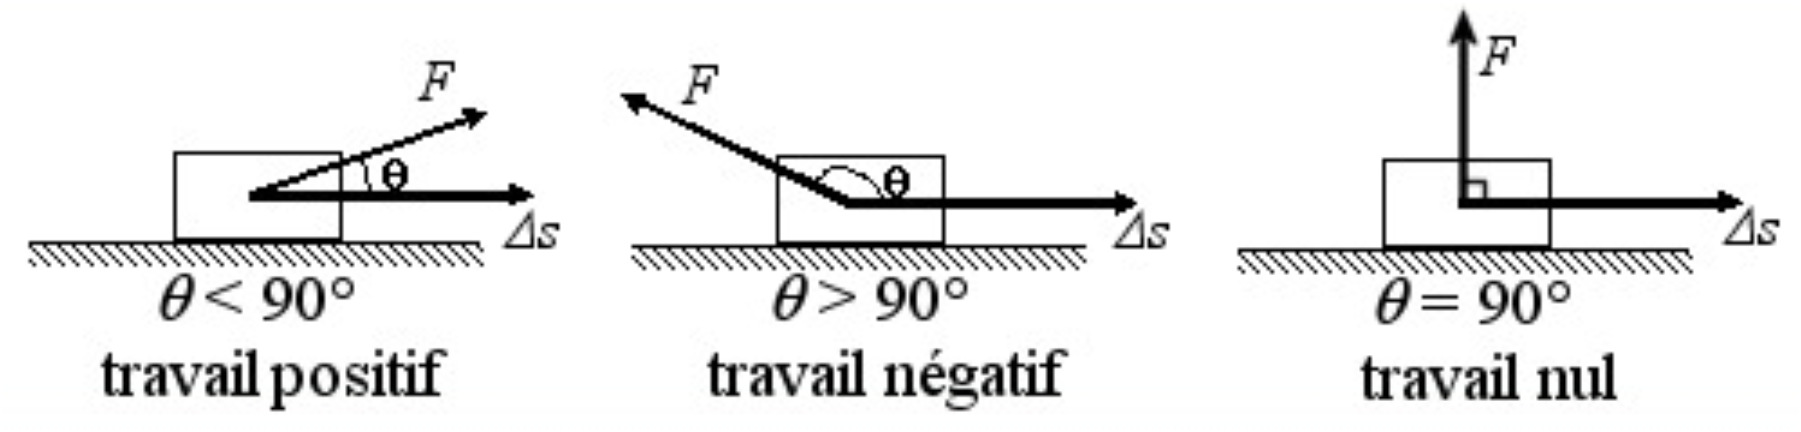
\includegraphics[width=12.989cm,height=3.115cm]{Pictures/1000000100000709000001B0D92B14C6C126C9B7.png}
\caption{}
\end{figure}

\begin{figure}
\centering
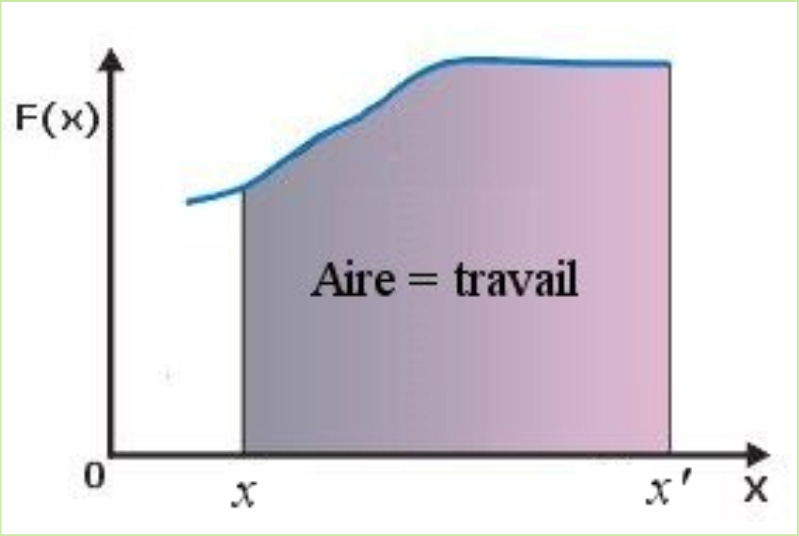
\includegraphics[width=7.292cm,height=4.895cm]{Pictures/100000010000031F00000218321A1B2B64E50C1E.png}
\caption{}
\end{figure}

(Sur le schéma~: $(x'-x) = \delta$) FIXME à mettre au bon endroit)

\subsection{Énergie}

\subsubsection{Définition}
On définit \textbf{ l'énergie est la capacité que
possède un corps à produire un travail. Son unité le Joule (J).}

La notion d'énergie est sans doute la plus importante de la physique. 
TODO à expliquer

\subsubsection{Différentes formes d'énergie~: }
\begin{itemize}
\item cinétique liée à la vitesse et à la masse d'un corps
\item potentielle liée à la masse d'un corps et à la hauteur à laquelle il
se trouve. (g est l'accélération de pesanteur).
\item mécanique égale la somme : Ecinétique + Epotentielle
\item thermique liée à la température d'un corps
\item électrique liée à l'électricité
\item chimique liée aux liaisons chimiques entre les atomes
\item rayonnante liée aux ondes électromagnétiques : la lumière,
l'infrarouge, l'ultraviolet etc.
\item nucléaire liée aux liaisons des protons et neutrons dans les noyaux
d'atomes
\item de masse liée à la masse selon la relation d'Einstein : $E = m c^2$, 
la formule sans doute la plus connue de tous, mais sans doute aussi mal 
comprise.
\end{itemize}



\subsection{Puissance }

En \href{https://fr.wikipedia.org/wiki/Physique}{physique},
la puissance reflète la vitesse à laquelle un
\href{https://fr.wikipedia.org/wiki/Travail_d\%27une_force}{\emph{\emph{travail}}}
est fourni.

\emph{Définition}~: C'est la quantité
d'\href{https://fr.wikipedia.org/wiki/\%C3\%89nergie_(physique)}{\emph{\emph{énergie}}}
fournie par unité de temps.

Son unité est le watt (\si{w}) (Remarque~: ne confondez pas le travail (W) et
le watt (\si{w}).

La puissance est une grandeur scalaire.

La puissance correspond donc à un débit d'énergie~: si deux systèmes de
puissances différentes fournissent \textbf{le même
}\href{https://fr.wikipedia.org/wiki/Travail_d\%27une_force}{travail},
\textbf{le plus puissant des deux est celui qui est le plus rapide.}




\subsection{Rendement }

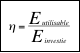
\includegraphics[width=3.108cm,height=2.073cm]{Pictures/10000001000000500000003510F712318EAE4AA8.png}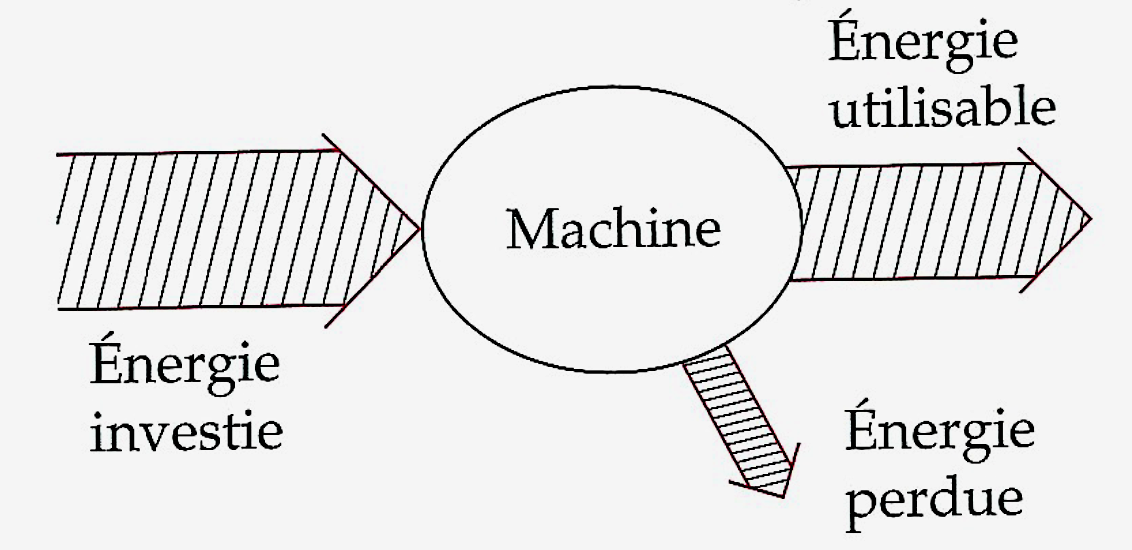
\includegraphics[width=5.011cm,height=2.441cm]{Pictures/100000010000046C00000226E09CB53258956B76.png}L'énergie
utilisable est la part de l'énergie finale \textbf{réellement exploitée}
pour satisfaire le besoin de l'usager.

Ce rapport est toujours inférieur à 1 (100 \%).

Un rendement de 100\% signifie qu'il n'y a aucune perte d'énergie.

\subsection{Des ordres de grandeur }
La liste ci-dessous reprend des ordres de grandeur d'énergie à connaître par cœur.
L'énergie de
\begin{itemize}
  \item un photon dans le domaine visible ≈ 10\textsuperscript{-19}
J
  \item un électron dans un tube TV ≈ 10\textsuperscript{-15 }J
  \item une pomme en chute libre ≈ 1 J
  \item une balle de tennis ≈ 10\textsuperscript{2} J
  \item une balle de fusil ≈ 10\textsuperscript{4} J
  \item chauffage de l'eau d'un bain ≈ 10\textsuperscript{7} J
  \item travail journalier d'un homme ≈ 10\textsuperscript{7} J
  \item une bombe d'une tonne de TNT ≈ 10\textsuperscript{10} J
  \item un éclair (de la foudre) ≈ 10\textsuperscript{10 }J
  \item consommée quotidiennement en Suisse ≈ 10\textsuperscript{14} J
  \item une bombe H (100 mégatonnes) ≈ 10\textsuperscript{18 }J
  \item une éruption solaire ≈ 10\textsuperscript{24} J
  \item d'une explosion de supernova ≈ 10\textsuperscript{40} J
\end{itemize}

La puissance est l'énergie produite ou dissipée par unité de temps, $P = \frac{E}{\Delta t}$. 
L'unité du SI de puissance est le Watt, $\si{w}$. 

TODO rajouter biographie de Watt et origine du WATT.

Quelques ordres de grandeur de puissances sont importantes à connaître~:
\begin{itemize}
  \item  dégagée par un corps humain au repos ≈ 70 à 100 w
  \item  consommée par un récepteur TV ≈ 100 w
  \item  consommée par un vélomoteur de 50 cm3 ≈ 900 w
  \item  consommée par un brûleur butane ≈ 900 w
  \item  consommée par un sèche-cheveux ≈ 1000 à 1300 w
  \item  consommée par une plaque électrique ≈ 1,5 kw
  \item  dégagée par un corps humain en activité ≈ 300 à 2000 w
  \item  consommée par séchoir à linge ≈ 5.10\textsuperscript{3} w à
8.10\textsuperscript{3} w
  \item  consommée par une voiture de tourisme (1400
cm\textsuperscript{3}) ≈ 40 kw
  \item  consommée par une locomotive électrique ≈ 5 Mw
  \item  dégagée par une centrale nucléaire (Doel) ≈ 3000 Mw
\end{itemize}


\subsection{Exercices}

\subsubsection*{Exercice 1}

Une voiture de 1,2 tonne et d'une puissance de 3000 watts atteint une
vitesse de 21,6 km/h en 10 secondes sur une route horizontale.
\begin{enumerate}
  \item   Quelle est l'énergie consommée ?
  \item   Quel sera le rendement~?
\end{enumerate}

\subsubsection*{Exercice 2}
\begin{enumerate}
  \item Quelle est l'énergie cinétique d'une voiture d'une tonne roulant à 72
km/h ?
   \item Quel travail faut-il effectuer pour arrêter cette voiture ?
\end{enumerate}

\subsubsection*{Exercice 3 }

Quelle est l'énergie consommée si on fournit une puissance de 2000 watts
pendant une minute ?

\subsubsection*{Exercice 4}

\begin{enumerate}
\item   Quelle est l'énergie potentielle d'un plongeur de 75 kg sur le
  plongeoir des 10 mètres ?
\item   En négligeant les frottements, quelle est son énergie cinétique à
  l'arrivée dans l'eau ?
\item   En négligeant le frottement, quelle est sa vitesse en arrivant dans
  l'eau, 10 mètres plus bas ?
\item   En négligeant le frottement, quelle est son énergie mécanique sur le
  plongeoir et à l'arrivée dans l'eau ?
\end{enumerate}

\subsubsection*{Exercice 5}

Une force de 12 N tire un chariot placé sur des rails. L'angle entre la
force et le sens des rails (et donc du déplacement) est de 30°. Quel est
le travail accompli si le chariot se déplace de 14m~?

\subsubsection*{Exercice 6}

Un haltérophile peut arracher du sol une masse de 183 kg et le soulever
à une hauteur de 2,1 m en 2 secondes. Quelle est la puissance
développée~?

\subsubsection*{Exercice 7}

Un wagon a une masse de 20 tonnes.

\begin{enumerate}
\item   Quelle force motrice faut-il lui appliquer pour qu'il atteigne une
  vitesse de 54 km/h au bout de 5minutes~?
\item   Quel sera le déplacement correspondant~?
\item   Quelle est la puissance du moteur~?
\end{enumerate}

%\end{multicols}

\subsection{Résolutions}

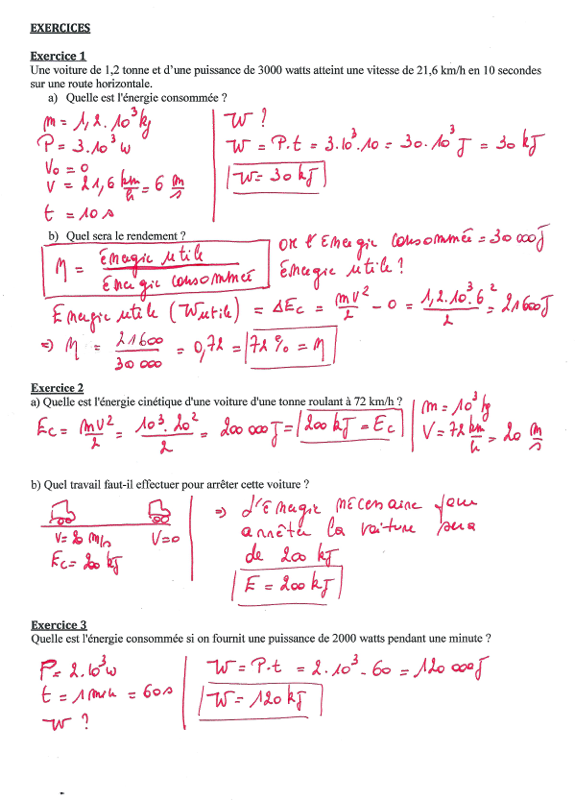
\includegraphics[width=16cm]{Pictures/100000010000023F00000321650A721E7772A454.png}

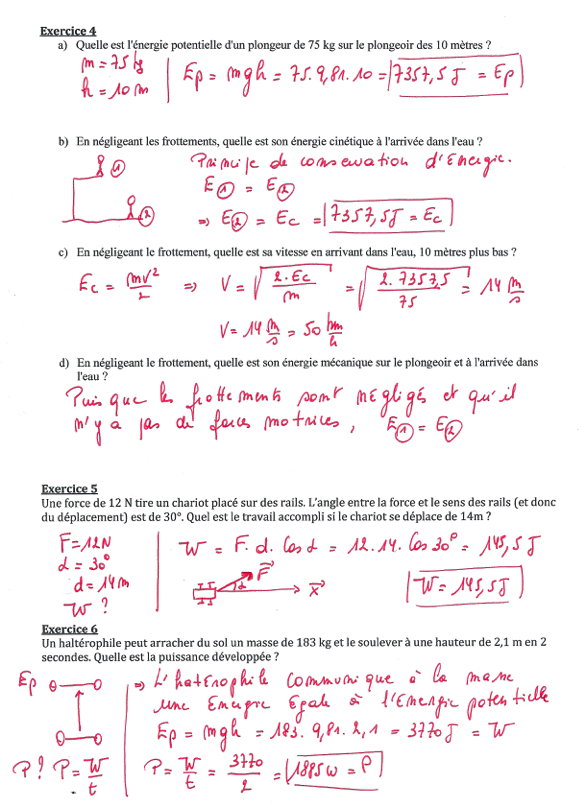
\includegraphics[width=16cm]{Pictures/100000010000024A00000328B79BD0C63CC6F682.png}

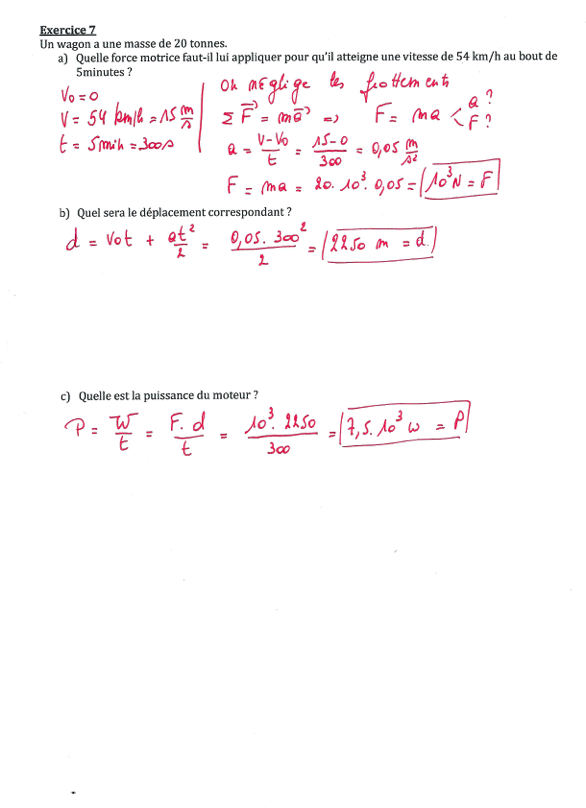
\includegraphics[width=16cm]{Pictures/100000010000024A0000032885BF0DEB477D1AAA.png}


